% !TEX root = ../main.tex
\section{QUY TRÌNH ELT, LAKEHOUSE, DBT VÀ PHÁT HÀNH KHO}
\suppressfloats[t]

Chương 4 đã cố định mô hình; còn thiếu cơ chế biến chín tệp CSV thành mô hình đó, theo cách có thể chạy lại và kiểm tra. Chương này mô tả 26 đợt nạp, 11 phép đối soát mỗi đợt, đường dựng thứ hai bằng dbt, và quy trình phát hành kho theo bản.

\subsection{Nạp theo 26 đợt tháng}
Tệp \texttt{orders} của Olist chỉ có trạng thái cuối cùng. Để kho có lịch sử như một hệ thống chạy thật, \texttt{src/etl/build.py} giả lập nguồn gửi dữ liệu theo tháng:
\begin{itemize}
    \item \textbf{Đợt \texttt{init}:} nạp dữ liệu master (khách, seller, sản phẩm, tọa độ, bản dịch danh mục): 1.135.721 dòng, cách ly 42 dòng.
    \item \textbf{26 đợt tháng} từ \texttt{2016-09} đến \texttt{2018-10}. Đợt tháng $m$ có mốc chốt $c$ là 00:00 ngày đầu tháng $m+1$.
\end{itemize}

\subsubsection*{Quy tắc point-in-time (\texttt{src/sql/10\_batch\_raw.sql})}
Tại mốc $c$ của mỗi đợt:
\begin{enumerate}
    \item Chỉ nhìn thấy đơn có thời điểm mua $< c$.
    \item Trạng thái được tái dựng từ các mốc đã xảy ra trước $c$: có ngày nhận $< c$ thì là \texttt{delivered}; có ngày giao vận chuyển $< c$ thì là \texttt{shipped}; có ngày duyệt $< c$ thì là \texttt{approved}; còn lại là \texttt{created}. Riêng \texttt{canceled} và \texttt{unavailable} giữ nguyên vì nguồn không có ngày hủy. Các mốc chưa xảy ra bị che thành NULL. Ở đợt cuối (\texttt{is\_final}), trạng thái nguồn được giữ nguyên; quy tắc tái dựng chỉ áp dụng cho các đợt giữa.
    \item Một phiên bản đơn mới chỉ được thêm vào \texttt{raw.orders} khi trạng thái hoặc một mốc thời gian đổi so với phiên bản trước. Kết quả là 137.236 phiên bản cho 99.441 đơn (1,38 phiên bản mỗi đơn).
    \item Review được nạp vào tháng khách trả lời (không sớm hơn tháng của đơn); dòng hàng và thanh toán được nạp vào tháng mua.
\end{enumerate}
Nhờ đó, mọi bảng chốt (\texttt{mart.*}, \texttt{fact\_seller\_monthly}) và mọi feature của DSS tại mốc $c$ chỉ dùng thông tin có trước $c$. Test hệ thống có một nhóm kiểm tra riêng cho điều này (Chương 8).

\subsubsection*{Nhật ký đợt}
\begin{figure}[htbp]
\centering
\begin{tikzpicture}
\begin{axis}[
    width=0.95\textwidth, height=5.6cm,
    ybar, bar width=5pt, ymin=0, ymax=36000, axis y line*=left,
    ylabel={Số dòng nạp trong đợt},
    xmin=0.3, xmax=26.7,
    xtick={2,5,8,11,14,17,20,23,26},
    xticklabels={Q4/16,Q1/17,Q2/17,Q3/17,Q4/17,Q1/18,Q2/18,Q3/18,Q4/18},
    minor xtick={1,...,26},
    major tick length=4pt, minor tick length=2pt,
    x tick label style={font=\scriptsize},
    xlabel={Đợt nạp theo tháng (nhãn chính: tháng đầu quý; vạch nhỏ: từng tháng)},
    ymajorgrids, grid style={gray!20},
    scaled y ticks=false, legend style={at={(0.3,1.03)}, anchor=south, draw=none},
]
\addplot[fill=hcmutnavy!60, draw=none] coordinates {(1,13) (2,1183) (3,175) (4,56) (5,2803) (6,7442) (7,11616) (8,10672) (9,16698) (10,14872) (11,17497) (12,19614) (13,19172) (14,20930) (15,30264) (16,29689) (17,31768) (18,30301) (19,34060) (20,33442) (21,32190) (22,28453) (23,27400) (24,31278) (25,734) (26,674)};
\addlegendentry{Số dòng}
\end{axis}
\begin{axis}[
    width=0.95\textwidth, height=5.6cm,
    ymin=0, ymax=3.6, axis y line*=right, axis x line=none, ylabel={Thời gian đợt (giây)},
    xmin=0.3, xmax=26.7,
    legend style={at={(0.7,1.03)}, anchor=south, draw=none},
]
\addplot[red!75!black, thick, mark=*, mark size=1.3pt] coordinates {(1,0.82) (2,1.1) (3,0.73) (4,1.0) (5,2.06) (6,0.89) (7,0.96) (8,1.25) (9,1.07) (10,1.73) (11,1.26) (12,1.81) (13,1.46) (14,1.77) (15,1.89) (16,2.2) (17,2.8) (18,2.63) (19,3.14) (20,3.33) (21,2.57) (22,3.1) (23,2.73) (24,3.29) (25,1.97) (26,2.47)};
\addlegendentry{Thời gian}
\end{axis}
\end{tikzpicture}
\caption{Số dòng nạp và thời gian của 26 đợt (\texttt{ops.etl\_log})}
\label{fig:batches}
\end{figure}

Hình~\ref{fig:batches} cho thấy mỗi đợt mất 0,73--3,33 giây, nhưng thời gian không tỷ lệ với số dòng: đợt 09/2018 chỉ nạp 734 dòng mà mất 1,97 giây, lâu hơn đợt 02/2017 (7.442 dòng, 0,89 giây). Nguyên nhân là bước đóng đợt (\texttt{12\_batch\_close.sql}) tính lại feature 90 ngày và KPI trên toàn bộ dữ liệu tích lũy, nên chi phí tăng theo kích thước kho chứ không theo kích thước đợt. Toàn bộ quá trình dựng kho — init, 26 đợt, ghi nhận bất thường, xuất Gold Parquet — mất 62,8 giây trên máy thử nghiệm. Ở quy mô Olist, chi phí đóng đợt chưa phải điểm nghẽn; với dữ liệu lớn hơn nhiều, bước đóng đợt nên chỉ tính trên cửa sổ 90 ngày thay vì toàn bộ lịch sử.

\subsection{Cổng chất lượng: 11 phép đối soát mỗi đợt}
Cuối mỗi đợt, \texttt{13\_batch\_}\allowbreak\texttt{checks.sql} so số dòng và số tiền giữa các lớp, ghi vào \texttt{ops.layer\_}\allowbreak\texttt{reconciliation} (Bảng~\ref{tab:recon}). Nếu có phép nào lệch, \texttt{run\_batch} ném \texttt{ReconciliationError}, ghi đợt là \texttt{failed}, và watermark không tiến; lần chạy sau sẽ chạy lại đợt đó.

\begin{table}[htbp]
\centering
\small
\caption{Mười một phép đối soát và giá trị ở đợt cuối (10/2018)}
\label{tab:recon}
\begin{tabularx}{\textwidth}{|>{\centering\arraybackslash}m{0.6cm}|>{\raggedright\arraybackslash}m{2.6cm}|L|>{\raggedleft\arraybackslash}m{2.6cm}|}
\hline
\textbf{\#} & \textbf{Đại lượng} & \textbf{Từ lớp $\rightarrow$ tới lớp} & \textbf{Giá trị (khớp)} \\
\hline
1 & Số đơn & \texttt{raw.orders} $\rightarrow$ \texttt{core.fact\_order} & 99.441 \\
\hline
2 & Số dòng hàng & \texttt{raw.order\_items} $\rightarrow$ \texttt{core.fact\_sales\_item} & 112.650 \\
\hline
3 & Số dòng thanh toán & \texttt{raw.order\_payments} $\rightarrow$ \texttt{core.fact\_payment} & 103.886 \\
\hline
4 & Số review & \texttt{raw.order\_reviews} $\rightarrow$ \texttt{core.fact\_review} & 99.224 \\
\hline
5 & Tiền hàng & \texttt{raw.order\_items} $\rightarrow$ \texttt{core.fact\_sales\_item} & 13.591.643,70 \\
\hline
6 & Tiền hàng & \texttt{core.fact\_sales\_item} $\rightarrow$ \texttt{core.fact\_order} & 13.591.643,70 \\
\hline
7 & Tiền hàng & \texttt{core.fact\_sales\_item} $\rightarrow$ \texttt{core.fact\_order\_seller} & 13.591.643,70 \\
\hline
8 & Tiền thanh toán & \texttt{raw.order\_payments} $\rightarrow$ \texttt{core.fact\_payment} & 16.008.872,12 \\
\hline
9 & GMV tháng & \texttt{core.fact\_sales\_item} $\rightarrow$ \texttt{mart.kpi\_monthly} & theo tháng \\
\hline
10 & GMV tháng & \texttt{core.fact\_sales\_item} $\rightarrow$ \texttt{core.fact\_seller\_monthly} & theo tháng \\
\hline
11 & GMV 90 ngày & \texttt{core.fact\_sales\_item} $\rightarrow$ \texttt{mart.seller\_features} & 770.146,48 \\
\hline
\end{tabularx}
\end{table}

Qua 26 đợt có $11 \times 26 = 286$ dòng đối soát, \textbf{286/286 khớp}. GMV tháng ở đợt 10/2018 bằng 0 vì tháng đó không có đơn hợp lệ. Cổng này có kiểm tra ngược: test hệ thống xóa 1 dòng ở \texttt{fact\_sales\_item} trên một bản sao kho rồi chạy lại đợt cuối, và đợt bị dừng với thông báo lệch ``số dòng hàng'' (Chương 8).

Các kiểm tra về cấu trúc (khóa chính, khóa ngoại mồ côi, SCD2 không chồng khoảng, mỗi seller một dòng \texttt{is\_current}) không nằm trong cổng đợt mà nằm trong \texttt{tests/test\_system.py}, chạy một lần sau khi dựng xong.

\subsection{Lakehouse Parquet đi kèm bản kho}
\texttt{src/etl/lakehouse.py} xuất dữ liệu ra Parquet nén ZSTD trong thư mục \texttt{<bản kho>\_lake/} cạnh tệp DuckDB:
\begin{itemize}
    \item \textbf{Bronze:} 5 tệp master (đợt \texttt{init}) và $26 \times 4 = 104$ tệp giao dịch theo đợt, phân vùng theo bảng (\texttt{bronze/orders/2017-11.parquet}, \dots). Tổng 109 tệp, 67,8 MB.
    \item \textbf{Gold:} 14 bảng dimension và fact, 33,4 MB.
\end{itemize}
Mỗi tệp Bronze được ghi một dòng vào sổ cái \texttt{ops.ingestion\_batches} gồm đợt, đường dẫn tệp, số dòng và \textbf{SHA-256 của chính tệp đó}: $9$ dòng cho các CSV của đợt \texttt{init} và $26 \times 4 = 104$ dòng cho các tệp Parquet, tổng 113 dòng. Nếu chạy lại một đợt, các dòng của đợt đó bị thay thế chứ không cộng dồn. Sổ cái cho phép kiểm tra sau này một tệp Parquet có bị sửa sau khi nạp hay không, bằng cách tính lại hash và so với sổ cái.

Thư mục lake gắn với một bản kho cụ thể (\texttt{olist\_x.duckdb} $\rightarrow$ \texttt{olist\_x\_lake/}) chứ không dùng một thư mục chung. Như vậy, khi một lần dựng bị hỏng hoặc khi quay lui (mục~\ref{sec:release}), Parquet và kho không lệch nhau. Test \texttt{tests/test\_lakehouse\_medallion.py} (11 kiểm tra) xác nhận:
\begin{itemize}
    \item đủ số tệp;
    \item \texttt{fact\_sales\_item} trong Parquet có cùng số dòng (112.650) và tổng tiền (13.591.643,70) với kho;
    \item sổ cái có đủ 113 dòng;
    \item 42 bản ghi cách ly có mã lỗi và payload.
\end{itemize}

\subsection{dbt: dựng lại kho bằng một đường thứ hai và đối chiếu}
Thư mục \texttt{dbt/} mô tả lại phép biến đổi Silver $\rightarrow$ Gold bằng 27 model SQL: 9 staging, 1 intermediate, 14 core, 3 mart. dbt đọc từ \texttt{raw} và ghi vào các schema riêng \texttt{dbt\_stg}, \texttt{dbt\_core}, \texttt{dbt\_mart}, nên \textbf{không bao giờ ghi đè} bảng \texttt{core} và \texttt{mart} mà ứng dụng và Power BI đang đọc. dbt mang lại hai thứ mà pipeline SQL theo đợt không có:
\begin{enumerate}
    \item \textbf{Đồ thị phụ thuộc (lineage)} giữa các model, sinh tự động từ \texttt{ref()}.
    \item \textbf{Một phép kiểm tra độc lập:} cùng dữ liệu \texttt{raw}, hai cách dựng (theo đợt bằng Python + SQL, và dựng một lần bằng dbt) phải ra cùng kết quả. Test \texttt{assert\_core\_matches\_python} so 11 đại lượng (Bảng~\ref{tab:dbt_check}).
\end{enumerate}

\begin{table}[htbp]
\centering
\small
\caption{Đối chiếu kho chính (\texttt{core}) với bản dbt dựng lại (\texttt{dbt\_core})}
\label{tab:dbt_check}
\begin{tabularx}{\textwidth}{|L|>{\raggedleft\arraybackslash}m{3.1cm}|>{\raggedleft\arraybackslash}m{3.1cm}|>{\centering\arraybackslash}m{1.3cm}|}
\hline
\textbf{Đại lượng} & \textbf{\texttt{core}} & \textbf{\texttt{dbt\_core}} & \textbf{Khớp} \\
\hline
Số dòng \texttt{fact\_sales\_item} & 112.650 & 112.650 & \checkmark \\
\hline
Tổng tiền \texttt{fact\_sales\_item} & 13.591.643,70 & 13.591.643,70 & \checkmark \\
\hline
Số dòng \texttt{fact\_order} / \texttt{fact\_order\_seller} & 99.441 / 100.785 & 99.441 / 100.785 & \checkmark \\
\hline
Tổng thanh toán \texttt{fact\_payment} & 16.008.872,12 & 16.008.872,12 & \checkmark \\
\hline
Số dòng \texttt{fact\_review} & 99.224 & 99.224 & \checkmark \\
\hline
Số dòng \texttt{dim\_customer} / \texttt{dim\_product} & 96.097 / 32.952 & 96.097 / 32.952 & \checkmark \\
\hline
Số dòng \texttt{dim\_seller} / \texttt{dim\_route} & 11.209 / 622 & 11.209 / 622 & \checkmark \\
\hline
ZIP có thành phố hoặc bang khác nhau & \multicolumn{2}{c|}{0 trên 19.178 ZIP} & \checkmark \\
\hline
\end{tabularx}
\end{table}

\subsubsection*{Phân tích thực nghiệm về hiệu quả của cơ chế kiểm tra chéo độc lập}
Thực nghiệm kiểm tra chéo độc lập đã chứng minh tính hữu hiệu thông qua việc phát hiện và cô lập lỗi phình to dữ liệu (Data Fan-out) do quan hệ 1--N trên dimension biến đổi chậm SCD Type 2. Trong lần tích hợp dbt vào chuỗi phát hành đầu tiên, \texttt{dbt\_core.fact\_sales\_item} sinh ra 513.492 dòng so với 112.650 dòng của kho chính, tức hệ số khuếch đại 4,56. Phân tích nguyên nhân cho thấy model dbt nối \texttt{dim\_seller} chỉ theo khóa tự nhiên \texttt{seller\_id}. Vì \texttt{dim\_seller} là SCD2 với trung bình 3,62 phiên bản mỗi seller, phép nối này có bản số 1--N và nhân mỗi dòng hàng theo số phiên bản của seller tương ứng. Pipeline chính sử dụng phép nối theo khoảng hiệu lực (point-in-time join):
\begin{equation}
\text{seller\_id}_f = \text{seller\_id}_d \;\land\; \text{valid\_from}_d \le \text{purchase\_ts}_f < \text{valid\_to}_d
\end{equation}
bảo đảm mỗi dòng sự kiện khớp đúng một phiên bản. Sau khi áp dụng cùng điều kiện cho model dbt, cả 11 đại lượng ở Bảng~\ref{tab:dbt_check} trùng khớp tuyệt đối. Cũng nhờ phép đối chiếu ở mức từng ZIP, nhóm phát hiện thêm một sai lệch thứ hai: bản sửa của pipeline chính về thứ tự xác định của hàm \texttt{mode()} khi hai tên thành phố có cùng tần suất chưa được đồng bộ sang dbt. Điểm đáng chú ý là cả hai lỗi đều \emph{không} bị phát hiện bởi bộ kiểm thử riêng của từng đường dựng; chỉ phép so sánh giữa hai cách hiện thực độc lập mới làm lộ ra chúng.

Phạm vi đối chiếu có giới hạn: các model tháng và mart của dbt (\texttt{fact\_seller\_monthly}, \texttt{kpi\_monthly}, \texttt{seller\_features}) là phiên bản rút gọn. Chúng chỉ tính ở mốc cuối thay vì chốt theo từng đợt, ví dụ \texttt{fact\_seller\_monthly} có 16.308 dòng so với 25.487. Vì vậy các bảng này \emph{không} được so. Tổng cộng \texttt{dbt build} chạy 27 model và 52 test, \textbf{79/79 đạt}.

\subsection{Phát hành kho theo bản}
\label{sec:release}
Ứng dụng giữ tệp DuckDB ở chế độ chỉ đọc, và DuckDB không cho tiến trình khác mở tệp đó để ghi. Nếu dựng lại kho bằng cách ghi đè lên tệp đang phục vụ, người dùng buộc phải dừng ứng dụng, đồng thời bất kỳ sai sót nào trong tiến trình nạp theo đợt đều có nguy cơ làm tổn hại tính sẵn sàng và tính toàn vẹn của kho dữ liệu phục vụ. Hệ thống tránh cả hai bằng các bản phát hành (\texttt{src/pipeline/release.py}, Hình~\ref{fig:release}):

\begin{figure}[htbp]
\centering
\resizebox{\textwidth}{!}{% Hình 5.2 -- Quy trình dựng và phát hành một bản kho
% Bốn bước ngang; mỗi bước có panel con ngay bên dưới, không chồng lấn.
\begin{tikzpicture}[font=\erdfont\scriptsize]
\kcard[minimum height=2.3cm]{c1}{0,0}{kdss}{3.1cm}{kfile}{1 \textperiodcentered{} Tạo bản mới}{%
  Tệp DuckDB mới trong \texttt{releases/}\\ chưa đổi \texttt{current.json}}
\kcard[minimum height=2.3cm]{c2}{3.9,0}{kdss}{3.1cm}{kdb}{2 \textperiodcentered{} Dựng kho}{%
  26 đợt + lake Parquet\\ DSS và catalog}
\kcard[minimum height=2.3cm]{c3}{7.8,0}{kdss}{3.1cm}{kshield}{3 \textperiodcentered{} Kiểm tra}{%
  Bốn cổng bên dưới\\ tất cả phải đạt}
\kcard[minimum height=2.3cm]{c4}{11.7,0}{kdss}{3.1cm}{kcheck}{4 \textperiodcentered{} Phát hành}{%
  Đổi \texttt{current.json}\\ bằng \texttt{os.replace}}

\foreach \a/\b in {c1/c2, c2/c3, c3/c4} \draw[karrow] (\a.east) -- (\b.west);

% ---- cột 3: bốn cổng và nhánh lỗi ----
\kcard[minimum height=2.2cm]{gates}{7.8,-2.55}{kwarn}{3.1cm}{kshield}{Bốn cổng}{%
  286 đối soát \textperiodcentered{} 133 test\\ 11 lakehouse \textperiodcentered{} 79 dbt}
\kcard[minimum height=2.3cm]{fail}{7.8,-5.15}{kalert}{3.1cm}{kcross}{Khi một cổng lỗi}{%
  Dừng ngay\\ \texttt{current.json} không đổi\\ app đọc bản đang dùng}
\draw[karrow] (c3.south) -- (gates.north);
\draw[kdash=kalert] (gates.south) -- (fail.north) node[midway, right, font=\erdfont\tiny, text=kalert] {lỗi};

% ---- cột 4: phát hành và quay lui ----
\kcard[minimum height=2.0cm]{curr}{11.7,-2.55}{klake}{3.1cm}{kcheck}{\texttt{current.json}}{%
  \texttt{os.replace} nguyên tử\\ app đọc bản mới ở lần tải sau}
\kcard[minimum height=2.0cm]{roll}{11.7,-5.15}{ksrc}{3.1cm}{kclock}{Quay lui}{%
  \texttt{rollback} đổi chỗ hai bản\\ bản cũ hơn bị xóa kèm lake}
\draw[karrow] (c4.south) -- (curr.north);
\draw[kdash=ksrc] (curr.south) -- (roll.north);

% ---- chân hình ----
\begin{scope}[yshift=-8.0cm]
  \draw[karrow] (0,0) -- (0.55,0);
  \node[anchor=west, font=\erdfont\tiny] at (0.6,0) {tiến trình};
  \draw[kdash=kalert] (3.1,0) -- (3.65,0);
  \node[anchor=west, font=\erdfont\tiny] at (3.7,0) {lỗi/quay lui};
  \node[anchor=west, font=\erdfont\tiny] at (7.2,0) {Mỗi bước chạy trong một tiến trình con trỏ vào bản phát hành của lần chạy đó};
\end{scope}
\end{tikzpicture}
}
\caption{Quy trình dựng và phát hành một bản kho; \texttt{run\_all.py} và Dagster dùng cùng tiêu chuẩn. Số 1--4 là thứ tự; nhánh nét đứt là lỗi/quay lui}
\label{fig:release}
\end{figure}

\begin{itemize}
    \item Mỗi lần dựng tạo một tệp mới trong \texttt{warehouse/releases/}.
    \item Chỉ khi mọi kiểm tra đạt, con trỏ \texttt{current.json} mới được đổi bằng một lần đổi tên nguyên tử (\texttt{os.replace}). Ứng dụng chỉ có thể thấy con trỏ cũ hoặc con trỏ mới, không bao giờ thấy tệp đang viết dở. Lần tải trang sau, ứng dụng đọc bản mới.
    \item Hệ thống giữ bản đang dùng và bản trước; lệnh \texttt{rollback} đổi chỗ hai bản. Bản cũ hơn được xóa kèm thư mục lake của nó.
    \item Mọi đường dẫn dữ liệu tính tương đối từ thư mục repo (\texttt{warehouse/}), nên chạy được trên máy khác mà không phải sửa cấu hình.
\end{itemize}
Bộ \texttt{tests/test\_release.py} (15/15 đạt) kiểm tra các tình huống trên một thư mục tạm:
\begin{itemize}
    \item phát hành được khi ứng dụng đang mở bản cũ;
    \item quay lui và quay lui lần nữa;
    \item từ chối tệp nằm ngoài \texttt{releases/} hoặc còn tệp \texttt{.wal};
    \item con trỏ hỏng thì quay về tệp mặc định.
\end{itemize}
Trong lúc phát triển, cơ chế này đã chặn đúng hai lần dựng lỗi: một lần do lỗi cú pháp YAML trong \texttt{catalog.yml}, một lần do lỗi phình to dữ liệu (fan-out) của dbt nêu ở trên. Cả hai lần, kho đang dùng không bị đổi.

\subsection{Điều phối bằng Dagster}
\texttt{src/pipeline/definitions.py} bọc các bước trên thành asset của Dagster, mỗi bước chạy trong một tiến trình con trỏ vào bản phát hành của lần chạy đó (Bảng~\ref{tab:dagster}). Logic không bị viết lại, nên số liệu giống \texttt{run\_all.py}. Dagster bổ sung giao diện xem từng bước, lịch sử chạy, log và lịch chạy hằng ngày lúc 02:00 (mặc định tắt).

\begin{table}[htbp]
\centering
\small
\caption{Asset và kiểm tra trong Dagster}
\label{tab:dagster}
\begin{tabularx}{\textwidth}{|>{\raggedright\arraybackslash\ttfamily}m{3.6cm}|>{\raggedright\arraybackslash}m{2.4cm}|L|}
\hline
\textbf{\rmfamily Asset / check} & \textbf{\rmfamily Loại} & \textbf{\rmfamily Nội dung} \\
\hline
nguon\_csv & Asset & Kiểm SHA-256 và số dòng 9 tệp \\
\hline
kho\_du\_lieu & Asset & Dựng kho 26 đợt và lake \\
\hline
doi\_soat\_cac\_lop & Check, chặn & Đủ 26 đợt \texttt{ok}, mọi dòng đối soát khớp \\
\hline
bat\_thuong\_du\_lieu & Check, cảnh báo & Liệt kê \texttt{dq\_issue} và số dòng cách ly \\
\hline
dss\_khuyen\_nghi & Asset & Mô hình, bảng luật, MILP, đánh giá \\
\hline
danh\_muc\_du\_lieu & Asset & Gắn mô tả cột từ \texttt{catalog.yml} \\
\hline
kiem\_thu\_he\_thong & Check, chặn & \texttt{tests.test\_system} \\
\hline
lakehouse\_va\_dbt & Check, chặn & Test lakehouse và \texttt{dbt build} \\
\hline
kho\_phat\_hanh & Asset & Đổi \texttt{current.json} \\
\hline
xuat\_parquet & Asset & Xuất 12 bảng cho Power BI từ bản đang dùng \\
\hline
\end{tabularx}
\end{table}

\subsubsection*{Đồ thị phụ thuộc và một lần chạy thực tế}
Hình~\ref{fig:dagster_lineage} là đồ thị phụ thuộc (DAG) của 6 asset trên giao diện Dagster, chia theo ba nhóm \texttt{kho}, \texttt{dss} và \texttt{phat\_hanh}. Viền xanh cho biết mọi asset đã được vật chất hóa (materialized) thành công ở lần chạy gần nhất. Vai trò của đồ thị này tương đương \emph{Graph View} trong Apache Airflow: mỗi node là một bước, mỗi cạnh là một phụ thuộc, và bước sau chỉ chạy khi bước trước thành công.

\begin{figure}[htbp]
\centering
\begin{tikzpicture}[dagimg/.style={inner sep=0pt, draw=gray!50, line width=0.4pt}]
\node[dagimg] (g1) {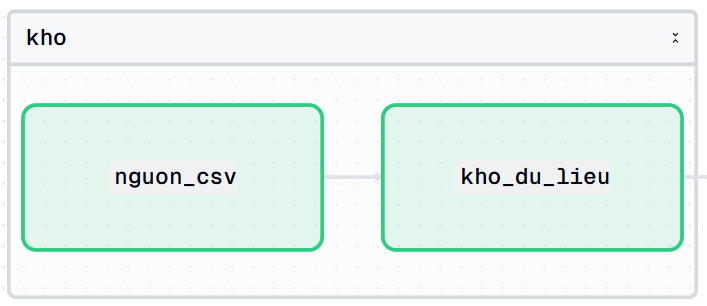
\includegraphics[width=0.62\textwidth]{image/dagster_1_kho.png}};
\node[dagimg, below=0.55cm of g1] (g2) {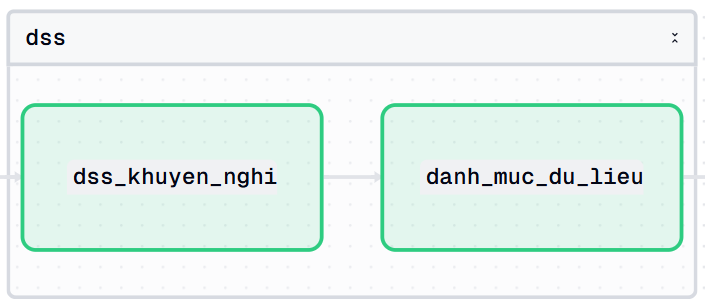
\includegraphics[width=0.62\textwidth]{image/dagster_1_dss.png}};
\node[dagimg, below=0.55cm of g2] (g3) {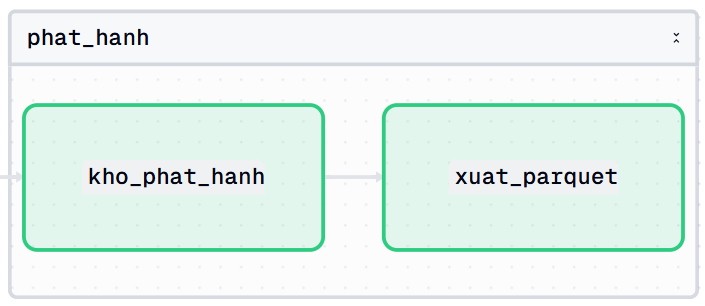
\includegraphics[width=0.62\textwidth]{image/dagster_1_phat_hanh.png}};
\draw[-{Stealth[length=2.6mm]}, line width=1pt, gray!70!black] (g1.south) -- (g2.north);
\draw[-{Stealth[length=2.6mm]}, line width=1pt, gray!70!black] (g2.south) -- (g3.north);
\end{tikzpicture}
\caption{Đồ thị phụ thuộc 6 asset trên Dagster (Global asset lineage), ba nhóm được xếp dọc để dễ đọc: kho $\rightarrow$ DSS $\rightarrow$ phát hành. Trong mỗi nhóm, asset bên trái chạy trước asset bên phải; viền xanh là đã chạy thành công}
\label{fig:dagster_lineage}
\end{figure}

Hình~\ref{fig:dagster_gantt} là biểu đồ Gantt của lần chạy job \texttt{dung\_lai\_toan\_bo} (mã \texttt{c0135898}), tương đương \emph{Gantt View} trong Airflow. Mỗi thanh là một bước, chiều dài là thời gian chạy:
\begin{itemize}
    \item Toàn bộ lần chạy mất \textbf{3 phút 14 giây}, cả \textbf{10/10 bước} thành công (6 asset và 4 kiểm tra), không bước nào lỗi.
    \item Bước dài nhất là \texttt{kho\_du\_lieu} (89 giây: dựng 26 đợt và lake), tiếp theo là kiểm tra \texttt{lakehouse\_va\_}\allowbreak\texttt{dbt} (38,5 giây, gồm test lakehouse và \texttt{dbt build}), \texttt{dss\_khuyen\_nghi} (18,6 giây: mô hình, MILP, đánh giá) và \texttt{kiem\_thu\_he\_thong} (15,5 giây).
    \item Hai kiểm tra \texttt{doi\_soat\_cac\_lop} và \texttt{bat\_thuong\_du\_lieu} chạy song song ngay sau khi kho dựng xong (khoảng 2 giây mỗi kiểm tra). Hai kiểm tra chặn \texttt{kiem\_thu\_he\_thong} và \texttt{lakehouse\_va\_dbt} cũng chạy song song; bước \texttt{kho\_phat\_hanh} (0,3 giây) chỉ bắt đầu khi cả hai đã đạt.
\end{itemize}
Lần chạy này phát hành bản kho \texttt{olist\_run\_c0135898.duckdb}. Bản này được đối chiếu với bản phát hành trước đó: số dòng và tổng tiền \texttt{fact\_sales\_item}, số phiên bản SCD2, số dòng cách ly, AUC và kế hoạch tại 01/07/2018 trùng khớp hoàn toàn, tức quy trình cho kết quả tái lập được (reproducible).

\appimage[0.98\textwidth]{image/dagster_4_run_gantt.png}{Biểu đồ Gantt lần chạy \texttt{dung\_lai\_toan\_bo} trên Dagster: 10 bước thành công trong 3 phút 14 giây}{fig:dagster_gantt}

Có ba job:
\begin{itemize}
    \item \texttt{dung\_lai\_toan\_bo}: chạy toàn bộ;
    \item \texttt{chay\_lai\_dss}: giữ kho, chép kho đang dùng kèm thư mục lake sang bản mới rồi chỉ tính lại DSS;
    \item \texttt{xuat\_power\_bi}: chỉ xuất lại Parquet.
\end{itemize}

\takeawaybox{Tóm tắt Chương 5}{
Ba lớp kiểm tra bổ sung cho nhau:
\begin{itemize}
    \item Đối soát theo đợt (286/286) bảo đảm không mất dòng, không lệch tiền giữa các lớp.
    \item Test hệ thống, test lakehouse và dbt bảo đảm cấu trúc đúng và hai cách dựng cho cùng kết quả.
    \item Cơ chế phát hành bảo đảm chỉ bản đã qua mọi kiểm tra mới tới tay người dùng.
\end{itemize}
Phép đối chiếu với dbt có giá trị thực tế: nó đã phát hiện một lỗi phình to dữ liệu (fan-out) với hệ số 4,56 mà các test của từng đường dựng riêng lẻ không bắt được.
}
